\documentclass[11pt]{article}

% Change "review" to "final" to generate the final (sometimes called camera-ready) version.
% Change to "preprint" to generate a non-anonymous version with page numbers.
\usepackage{acl}

% Standard package includes
\usepackage{times}
\usepackage{lipsum}
\usepackage{latexsym}
\usepackage{amsmath}
\usepackage{booktabs}
\hbadness=10000
\vbadness=10000

% For proper rendering and hyphenation of words containing Latin characters (including in bib files)
\usepackage[T1]{fontenc}
% For Vietnamese characters
% \usepackage[T5]{fontenc}
% See https://www.latex-project.org/help/documentation/encguide.pdf for other character sets

% This assumes your files are encoded as UTF8
\usepackage[utf8]{inputenc}

% This is not strictly necessary, and may be commented out,
% but it will improve the layout of the manuscript,
% and will typically save some space.
\usepackage{microtype}

% This is also not strictly necessary, and may be commented out.
% However, it will improve the aesthetics of text in
% the typewriter font.
\usepackage{inconsolata}

%Including images in your LaTeX document requires adding
%additional package(s)
\usepackage{graphicx}

% If the title and author information does not fit in the area allocated, uncomment the following
%
%\setlength\titlebox{<dim>}
%
% and set <dim> to something 5cm or larger.
\setlength\titlebox{13\baselineskip}

\title{SemEval-2026 Task 13: Detecting Machine-Generated Code with Multiple Programming Languages, Generators, and Application Scenarios}

% Author information can be set in various styles:
% For several authors from the same institution:
% \author{Author 1 \and ... \and Author n \\
%         Address line \\ ... \\ Address line}
% if the names do not fit well on one line use
%         Author 1 \\ {\bf Author 2} \\ ... \\ {\bf Author n} \\
% For authors from different institutions:
% \author{Author 1 \\ Address line \\  ... \\ Address line
%         \And  ... \And
%         Author n \\ Address line \\ ... \\ Address line}
% To start a separate ``row'' of authors use \AND, as in
% \author{Author 1 \\ Address line \\  ... \\ Address line
%         \AND
%         Author 2 \\ Address line \\ ... \\ Address line \And
%         Author 3 \\ Address line \\ ... \\ Address line}

\author{Sabrina Bonfante \\
  Politecnico di Torino \\
  Computer Engineering \\
  \texttt{s343496} \\\And
  Edoardo Cotto \\
  Politecnico di Torino \\
  Computer Engineering \\
  \texttt{s343449} \\\And
  Iulian Lucian Andro \\
  Politecnico di Torino \\
  Computer Engineering \\
  \texttt{s346481}\\\And
  Francesco Papini\\
  Politecnico di Torino \\
  Computer Engineering \\
\texttt{s336426}\\\AND
  \text{GitHub repository:} \url{https://github.com/papo1011/semeval2026}}
%\author{
%  \textbf{First Author\textsuperscript{1}},
%  \textbf{Second Author\textsuperscript{1,2}},
%  \textbf{Third T. Author\textsuperscript{1}},
%  \textbf{Fourth Author\textsuperscript{1}},
%\\
%  \textbf{Fifth Author\textsuperscript{1,2}},
%  \textbf{Sixth Author\textsuperscript{1}},
%  \textbf{Seventh Author\textsuperscript{1}},
%  \textbf{Eighth Author \textsuperscript{1,2,3,4}},
%\\
%  \textbf{Ninth Author\textsuperscript{1}},
%  \textbf{Tenth Author\textsuperscript{1}},
%  \textbf{Eleventh E. Author\textsuperscript{1,2,3,4,5}},
%  \textbf{Twelfth Author\textsuperscript{1}},
%\\
%  \textbf{Thirteenth Author\textsuperscript{3}},
%  \textbf{Fourteenth F. Author\textsuperscript{2,4}},
%  \textbf{Fifteenth Author\textsuperscript{1}},
%  \textbf{Sixteenth Author\textsuperscript{1}},
%\\
%  \textbf{Seventeenth S. Author\textsuperscript{4,5}},
%  \textbf{Eighteenth Author\textsuperscript{3,4}},
%  \textbf{Nineteenth N. Author\textsuperscript{2,5}},
%  \textbf{Twentieth Author\textsuperscript{1}}
%\\
%\\
%  \textsuperscript{1}Affiliation 1,
%  \textsuperscript{2}Affiliation 2,
%  \textsuperscript{3}Affiliation 3,
%  \textsuperscript{4}Affiliation 4,
%  \textsuperscript{5}Affiliation 5
%\\
%  \small{
%    \textbf{Correspondence:} \href{mailto:email@domain}{email@domain}
%  }
%}

\begin{document}
\maketitle

\begin{abstract}
  \textit{The rapid advancement of large language models for code generation has made distinguishing machine-generated code from human-written code increasingly challenging. SemEval-2026 Task 13 addresses this problem through multiple subtasks involving binary detection, authorship attribution, and hybrid code identification across different programming languages and domains.
  In this paper, we present our approach for the different subtasks:}

  \textbf{Subtask A:} \textit{We adopt a zero-shot Fast-DetectGPT approach based on analytic sampling discrepancy. Extending the original single-threshold formulation, we analyze both single and double threshold strategies to better capture the shape of discrepancy score distributions across domains. The best configuration uses Stable-Code-3B with a single threshold, achieving a Macro F1-score of 0.72.}

  \textbf{Subtask B:}\textit{ We investigate a transformer-based approach for multi-class code authorship detection. Our system fine-tunes UniXCoder, a pre-trained model for source code understanding, to distinguish human-written code from code generated by ten different large language model families. To mitigate the severe class imbalance of the dataset, we employ class-weighted Focal Loss during training. Our approach achieves a Macro F1-score of 0.372 and an accuracy of 67.70\%.}

  \textbf{Subtask C:} \textit{ Addresses the complex challenge of hybrid and adversarial code detection. We formulated this as a 4-class sequence classification problem, fine-tuning the pre-trained UniXcoder model. To effectively manage the varying distribution of human, machine, hybrid, and adversarial samples, our system incorporates a dynamically class-weighted Focal Loss function. Evaluated on the local test set, the proposed approach achieves an Macro F1-score of 0.84 and  Accuracy of 88.70\%, demonstrating a strong capability to isolate fine-grained generation and obfuscation }artifacts.
\end{abstract}

\section{Introduction}
Recent advances in generative artificial intelligence have transformed software development practices. Large Language Models (LLMs) for code generation are now capable of producing  syntactically correct and semantically meaningful source code across multiple programming languages and domains, and are increasingly integrated into real-world development environments through tools such as GitHub Copilot and ChatGPT.

The widespread adoption of these systems raises important challenges related to authorship attribution, academic integrity, plagiarism detection, software security, and trustworthiness. As machine-generated code becomes increasingly similar to human-written code, automatically identifying its origin becomes a challenging research problem.

SemEval-2026 Task 13 addresses this challenge through three complementary subtasks designed to evaluate the robustness and generalization capabilities of machine-generated code detection systems.


\textbf{Subtask A} focuses on binary machine-generated code detection, where the goal is to classify a code snippet as either human-written or fully machine-generated. The task evaluates system generalization across both seen and unseen programming languages and domains.

\textbf{Subtask B} extends the problem to multi-class authorship attribution. Instead of simply detecting whether code is machine-generated, systems must identify the specific family of large language models responsible for generating the code, including models such as DeepSeek, Qwen, OpenAI, Meta-LLaMA, and Mistral.

\textbf{Subtask C} further increases the complexity of the task by introducing hybrid and adversarial code samples. In this setting, systems must distinguish among human-written, machine-generated, hybrid, and adversarially generated code snippets designed to mimic human coding styles.


\section{Background}

\subsection{ Subtask A}

Zero-shot detectors distinguish machine-generated text using statistical signals from language models. DetectGPT \cite{mitchell2023detectgptzeroshotmachinegeneratedtext} introduced probability curvature, but relies on costly perturbation sampling. Fast-DetectGPT \cite{bao2024fastdetectgptefficientzeroshotdetection} makes this process more efficient through analytic sampling discrepancy based on conditional probability curvature. We adapt this approach to source code and extend it by comparing single and double threshold decision rules across different code domains.

\subsection{ Subtask B and C}

Among these models, UniXCoder \cite{guo2022unixcoderunifiedcrossmodalpretraining} has demonstrated strong performance across multiple code understanding tasks by jointly modeling programming languages and natural language descriptions. Given its ability to capture semantic information beyond lexical patterns, UniXCoder represents a suitable choice for the multi-class authorship detection problem addressed in Subtask B and C.

\section{System overview}
\subsection{Dataset}

We used the official SemEval-2026 Task 13 dataset provided through Hugging Face \cite{orel-etal-2025-codet, orel2025textttdroidresourcesuiteaigenerated}. The dataset is divided into three subtasks corresponding to different machine-generated code detection scenarios.

Each sample in the dataset contains the following fields: \texttt{code} (source code snippet), \texttt{generator} (source model or author of the code), \texttt{label} (target class label), \texttt{language} (programming language of the snippet).

The dataset includes code written in multiple programming languages. Both human-written and machine-generated code samples are provided. Machine-generated samples originate from several Large Language Model families such as OpenAI, Qwen, DeepSeek, Meta-LLaMA, BigCode, Gemma, Mistral, and others.

\subsubsection{ Subtask A}

Subtask A focuses on binary machine-generated code detection. The objective is to classify each code snippet as either: human-written, machine-generated.

The training set contains approximately 500K samples, while the validation set contains 100K samples. Training data is primarily composed of algorithmic programming problems written in Python, Java, and C++. Evaluation settings additionally include unseen programming languages and unseen domains such as research and production code.

\subsubsection{ Subtask B}

Subtask B extends the task to multi-class authorship detection. Instead of binary classification, systems must identify the author category associated with each code snippet.

The dataset includes one human class together with multiple LLM families, including:

DeepSeek-AI, Qwen, 01-ai, BigCode, Gemma, Phi, Meta-LLaMA, IBM-Granite, Mistral, OpenAI.

The training split contains approximately 500K samples, while the validation split contains 100K samples.

\subsubsection{ Subtask C}

Subtask C focuses on hybrid code detection. The objective is to classify each snippet into one of four categories: human-written, machine-generated, hybrid, adversarial.

Hybrid samples correspond to partially AI-generated code, while adversarial samples are intentionally designed to mimic human coding behavior.

The training set contains approximately 900K samples and the validation set contains 200K samples.

\subsection{Architecture}
\subsubsection{Subtask A}

We adopt a training-free zero-shot architecture based on Fast-DetectGPT \cite{bao2024fastdetectgptefficientzeroshotdetection}. Each input code snippet is processed by a code-oriented LLM, which provides token-level probability distributions through its logits.

These probabilities are used to compute the analytic sampling discrepancy score, which can be interpreted as a normalized deviation of the observed sequence from the model's expected behavior. Specifically, the score compares the log-probability of the input sequence with the expected log-probability under the model distribution, normalized by the corresponding standard deviation. In this sense, the discrepancy score measures how many standard deviations the observed sequence lies above or below the model's expected log-probability. Since the required mean and variance can be computed directly from the model probabilities, the architecture avoids explicit perturbation generation and additional sampling steps.


The final prediction is obtained through a threshold-based decision rule.


\subsubsection{ Subtask B} Our approach fine-tunes UniXCoder \cite{guo2022unixcoderunifiedcrossmodalpretraining} for multi-class code authorship classification. Each source code snippet is tokenized using the official UniXCoder tokenizer and encoded by the transformer backbone. The resulting sequence representation is processed by a classification layer that assigns the input to one of eleven classes, corresponding to human-written code or one of ten LLM families.

Given the highly imbalanced class distribution of the dataset, we replace the standard cross-entropy objective with a class-weighted Focal Loss \cite{lin2018focallossdenseobject}, which increases the contribution of minority classes during training. Model selection is performed using the validation Macro F1-score, while early stopping is applied to reduce overfitting.

The prediction pipeline can be summarized as follows:

Code Snippet → UniXCoder Tokenizer → UniXCoder Encoder → Classification Head → Author Label

\subsubsection{ Subtask C}
Similar to Subtask B, we formulate Subtask C as a 4-class sequence classification problem using the UniXCoder \cite{guo2022unixcoderunifiedcrossmodalpretraining} model. The architecture processes tokenized code snippets through the transformer backbone, passing the resulting sequence representations to a classification head configured to predict one of four categories: human, machine, hybrid, or adversarial. To handle the disparate sample distributions across these four classes, we also integrate a dynamically class-weighted Focal Loss \cite{lin2018focallossdenseobject} function into the architecture.

The prediction pipeline follows the same structure of Subtask B.

\subsection{Methodology}
\subsubsection{ Subtask A}
We first compute a discrepancy score for each sample using the analytic sampling discrepancy formulation. Threshold calibration is then performed on a balanced subset of the training set, containing the same number of human-written and machine-generated samples. The decision thresholds are selected by maximizing Macro F1-score, which is the main evaluation metric of the task.

We compare two thresholding strategies:
\begin{itemize}
  \item \textbf{Single threshold:} this strategy follows the original Fast-DetectGPT \cite{bao2024fastdetectgptefficientzeroshotdetection} formulation. A snippet is classified as machine-generated when its discrepancy score exceeds a single calibrated threshold.
  \item \textbf{Double threshold:} this strategy extends the original formulation by jointly optimizing a lower and an upper threshold. A snippet is classified as machine-generated when its score falls outside the human-typical region, either below the lower threshold or above the upper threshold.

    {\small
      \[
        \operatorname{Predic}(x) =
        \begin{cases}
          1 \; (\text{AI}) &
          \begin{aligned}[t]
            \text{if } & Z(x) > \tau_{\text{upper}} \text{ or} \\
            & Z(x) < \tau_{\text{lower}},
          \end{aligned} \\
          0 \; (\text{Human}) & \text{otherwise.}
        \end{cases}
      \]
    }
\end{itemize}

Finally, we analyze the resulting score distributions to compare the behavior of the two thresholding strategies across the seen algorithmic training domain and the official mixed test setting.


\subsubsection{ Subtask B}
Code snippets are tokenized using the UniXCoder \cite{guo2022unixcoderunifiedcrossmodalpretraining} tokenizer and padded or truncated to a maximum sequence length of 512 tokens. The model is fine-tuned for multi-class classification, where each sample is assigned to one of eleven classes corresponding to human-written code or one of ten LLM families. Training is performed for 2 epochs using a batch size of 8 and mixed precision (FP16) when GPU resources are available. We optimize the network using a learning rate of $2\times10^{-5}$ and a weight decay of 0.01.

To address the severe class imbalance present in the dataset, balanced class weights are computed from the training distribution and incorporated into a Focal Loss \cite{lin2018focallossdenseobject} objective with a focusing parameter of $\gamma=2.0$. Early stopping with a patience of 2 evaluation rounds is employed during training, monitoring the validation Macro F1-score to select the best-performing model checkpoint.

\subsubsection{ Subtask C}
Code snippets are tokenized using the UniXcoder \cite{guo2022unixcoderunifiedcrossmodalpretraining} tokenizer and padded or truncated to a maximum sequence length of 512 tokens.
The model is fine-tuned for 3 epochs using a batch size of 64 and mixed precision (FP16) to maximize memory and training efficiency.
We optimize the network utilizing a learning rate of $2 \times 10^{-5}$ and a weight decay of 0.01.

To explicitly manage the class imbalance present in the dataset, we compute balanced class weights directly from the training distribution and apply them to a Focal Loss \cite{lin2018focallossdenseobject} function configured with a focusing parameter of $\gamma = 2.0$.
Early stopping with a patience of 2 epochs is employed during training, continuously monitoring the validation Macro F1-score to save and select the optimal model checkpoint.

\subsection{Model Selections}
\subsubsection{ Subtask A} 

\begin{table}[htbp]
  \centering
  \small
  \resizebox{\columnwidth}{!}{%
    \begin{tabular}{lc}
      \toprule
      \textbf{Model} & \textbf{Macro F1} \\
      \midrule
      Stable-Code-3B & 0.72 \\
      Starcoder2-7B & 0.71 \\
      CodeLlama-7B-hf & 0.70 \\
      Starcoder2-3B & 0.70 \\
      CodeLlama-7B-Instruct-hf & 0.68 \\
      CodeLlama-7B-Python-hf & 0.65 \\
      Qwen2.5-Coder-3B & 0.64 \\
      Qwen2.5-Coder-7B & 0.60 \\
      Qwen2.5-Coder-1.5B & 0.60 \\
      Yi-Coder-9B-Chat & 0.58 \\
      Yi-Coder-9B & 0.58 \\
      DeepSeek-Coder-1.3B-Base & 0.55 \\
      Qwen2.5-Coder-3B-Instruct & 0.54 \\
      Qwen2.5-Coder-7B-Instruct & 0.54 \\
      DeepSeek-Coder-6.7B-Base & 0.51 \\
      DeepSeek-Coder-1.3B-Instruct & 0.50 \\
      DeepSeek-Coder-6.7B-Instruct & 0.50 \\
      \bottomrule
    \end{tabular}
  }
  \caption{Model selection F1 results for zero-shot Fast-DetectGPT on Task A}
  \label{tab:model_comparison}
\end{table}

Model selection was guided by the Fast-DetectGPT setting \cite{bao2024fastdetectgptefficientzeroshotdetection}, where the scoring model directly affects the quality of the discrepancy score. Following the empirical observations of the original paper, we focused mainly on small language models, especially in the 1B--7B parameter range. This choice is also motivated by practical constraints, as smaller models reduce inference cost and GPU memory requirements while still providing effective probability estimates for detection.

We evaluated both models related to generator families present in the dataset and external code models not explicitly used as dataset generators. Interestingly, the best result was achieved by stable-code-3b, an external model, suggesting that generator-family overlap is not directly correlated with scoring effectiveness. We also did not observe a consistent relationship between model size and detection performance: StarCoder2-7B outperforms StarCoder2-3B, while Qwen2.5-Coder shows the opposite trend, with the 3B model performing better than the 7B variant. Overall, these results indicate that scoring effectiveness depends more on the shape and calibration of the model probability distribution over code than on size or generator-family overlap alone.


\subsubsection{ Subtask B and C}

UniXCoder \cite{guo2022unixcoderunifiedcrossmodalpretraining} was selected as the backbone model due to its strong performance on a variety of source code understanding tasks. Unlike lexical feature-based approaches, transformer architectures can capture contextual and semantic information within source code, enabling more effective modeling of programming patterns and coding styles.

The model was initialized from the publicly available \texttt{microsoft/unixcoder-base}\footnote{\url{https://huggingface.co/microsoft/unixcoder-base}} model and subsequently fine-tuned on the SemEval-2026 Task 13 dataset. To improve robustness against the highly imbalanced class distribution in Task B, we adopted a class-weighted Focal Loss \cite{lin2018focallossdenseobject} of the standard cross-entropy objective.

This combination allows the model to leverage rich code representations while improving learning for underrepresented author classes.

\subsection{Validation Strategy}
Following the shared task guidelines, Macro F1-score was adopted as the primary evaluation metric, as it equally weights all classes regardless of their frequency. In addition to Macro F1-score, we report accuracy, precision, and recall to provide a more comprehensive assessment of model performance.





%
%\subsection{Prompt-based Inference with Qwen3-Coder-Next}
%
%We evaluated a prompt-only approach using Qwen3-Coder-Next as a binary detector for Subtask A. Due to the memory and disk constraints of Google Colab Pro, we used the
%Unsloth quantized GGUF checkpoint \texttt{Qwen3-Coder-Next-UD-Q3\_K\_XL}, approximately 36.3GB, executed through \texttt{llama.cpp}. The model was served locally using
%\texttt{llama-server} and queried through an OpenAI-compatible chat-completion interface.
%
%For each example, the model received the programming language and code snippet, while the \texttt{generator} metadata was deliberately excluded to avoid label leakage.
%The prompt requested a JSON output with a binary label, where 0 denotes human-written code and 1 denotes machine-generated code. We used a few-shot prompting strategy
%with balanced examples from both classes. After an initial run showed a strong bias toward predicting machine-generated code, we revised the prompt to be more
%conservative: the model was instructed to predict machine-generated code only when clear generation artifacts were present, and to treat clean formatting, comments,
%boilerplate, bugs, or unusual style as insufficient evidence by themselves.
%
%The final prompt used four examples per class and emphasized signals such as explanatory prose inside code, markdown artifacts, placeholder implementations,
%inconsistent API usage, unused templated parameters, and code that describes a solution more than implementing it. Ambiguous cases were explicitly assigned to the
%human-written class.
%
%On a labeled 1,000-example test sample, the initial prompt achieved a macro F1 of 0.4516. After prompt refinement, macro F1 improved to 0.5591. The main improvement
%came from increased recall on human-written code, which rose from 0.3243 to 0.5212, while machine-generated recall remained relatively high at 0.7937.
%
%\subsection{Qwen3 Computational Cost}
%
%Qwen3-Coder-Next was run on NVIDIA A100 GPU in Google Colab Pro. The runtime cost for A100 usage is estimated to 5.3 compute units per hour. Building \texttt{llama.cpp},
%loading the quantized model, and running inference over the 1000 example sample took approximately 0.6 hours. Therefore, the total computational cost was 3.18 compute units. This cost includes both setup overhead and inference time.
%

\section{Experimental results}


\subsection{Subtask A}

Table~\ref{tab:model_comparison} reports the performance of the evaluated code-oriented language models using the Fast-DetectGPT \cite{bao2024fastdetectgptefficientzeroshotdetection} discrepancy score. The best result is obtained by \texttt{stable-code-3b}, which achieves a Macro F1-score of 0.7219.
\begin{figure}[h]
  \centering
  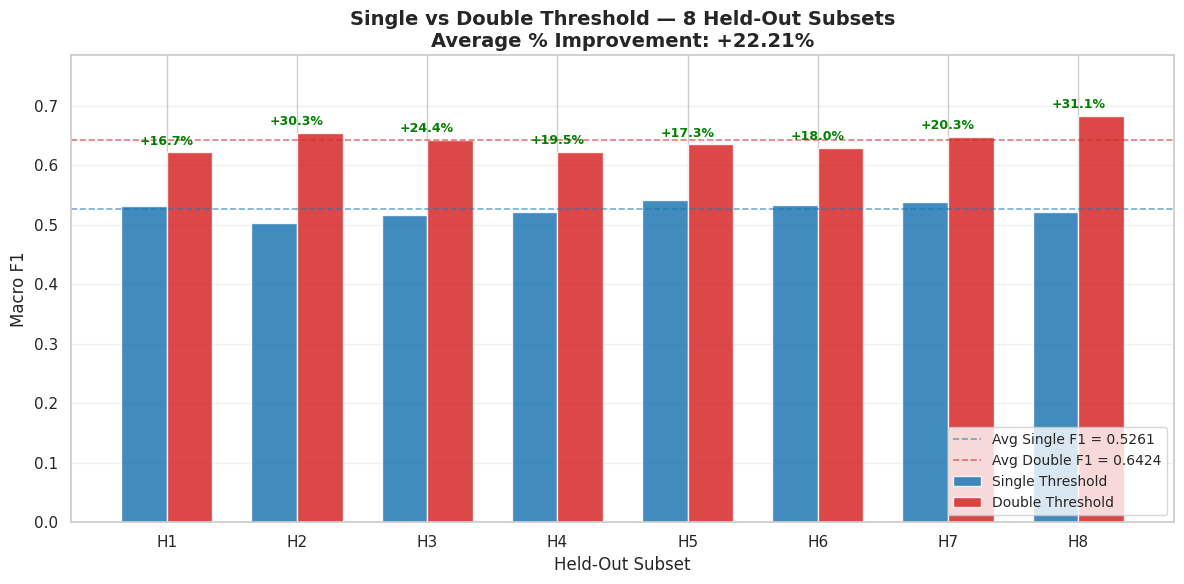
\includegraphics[width=\columnwidth]{assets/task_a_single_vs_double.png}
  \caption{Comparison between single and double threshold strategies on the LeetCode training domain.}
  \label{fig:single_vs_double_threshold}
\end{figure}
\paragraph{Training-domain analysis: LeetCode.}
We first analyze the thresholding strategies within the same domain used for calibration, namely the LeetCode-style algorithmic code domain. To make the comparison more stable, thresholds are fitted on a balanced training subset and then evaluated on multiple disjoint held-out subsets from the same training distribution. This allows us to measure whether the double-threshold strategy consistently improves over the original single-threshold rule when no domain shift is introduced.

In this setting, the double-threshold strategy clearly outperforms the single-threshold formulation. On average, the single threshold reaches a Macro F1-score of 0.5261, while the double threshold reaches 0.6424. This corresponds to an average absolute improvement of 0.1163 Macro F1 points, or a relative improvement of 22.21\%.



\begin{table}[htbp]
  \centering
  \small
  \caption{Average single and double threshold comparison on the LeetCode training domain.}
  \label{tab:leetcode_threshold_comparison}
  \resizebox{\columnwidth}{!}{%
    \begin{tabular}{lccc}
      \toprule
      \textbf{Strategy} & \textbf{Macro F1} & \textbf{Delta} & \textbf{Improvement} \\
      \midrule
      Single threshold & 0.53 & -- & -- \\
      Double threshold & 0.64 & +0.12 & +22.21\% \\
      \bottomrule
    \end{tabular}
  }
\end{table}

Figure~\ref{fig:threshold-train} explains why the double threshold is effective in this setting. In the LeetCode domain, human-written code is mostly concentrated in a central score region, while machine-generated code has a wider distribution with relevant mass in both tails. The upper tail captures highly predictable generated code, which is already detected by the single-threshold rule. However, the lower tail contains additional machine-generated samples with unusually low discrepancy scores. Since this lower tail is still relatively separated from the human distribution in the training domain, adding a lower threshold allows the detector to recover more machine-generated samples without introducing many false positives.

\begin{figure}[t]
  \centering
  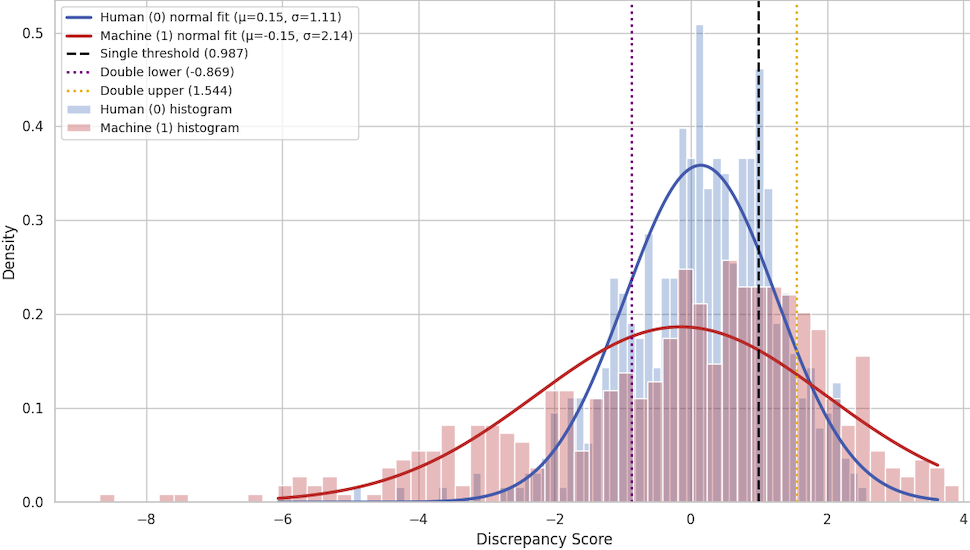
\includegraphics[width=\columnwidth]{assets/task_a_train.png}
  \caption{Double-threshold decision strategy on the LeetCode training domain using Stable-Code-3B.}
  \label{fig:threshold-train}
\end{figure}

\paragraph{Official test-set analysis.}
We then evaluate the same thresholding strategies after switching to the official Task A test setting, which includes a broader and more heterogeneous code distribution. In this case, the behavior changes substantially. The single-threshold strategy achieves the best result, with a Macro F1-score of 0.7219, while the double-threshold strategy drops to 0.5799.

\begin{table}[htbp]
  \centering
  \small
  \caption{Single and double threshold comparison on the official Task A test setting.}
  \label{tab:test_threshold_comparison}
  \resizebox{\columnwidth}{!}{%
    \begin{tabular}{lcccc}
      \toprule
      \textbf{Strategy} & \textbf{Accuracy} & \textbf{Precision} & \textbf{Recall} & \textbf{Macro F1} \\
      \midrule
      Single threshold & 0.82 & 0.75 & 0.71 & 0.72 \\
      Double threshold & 0.64 & 0.59 & 0.62 & 0.58 \\
      \bottomrule
    \end{tabular}
  }
\end{table}

The distribution in Figure~\ref{fig:threshold-test} shows why the double threshold does not transfer well to the mixed test distribution. Unlike the LeetCode-domain setting, the lower tail is no longer a reliable indicator of machine-generated code. Human-written snippets from generic code domains can also receive very low discrepancy scores, producing a much stronger overlap with the machine-generated distribution. As a consequence, the lower threshold captures some additional generated samples, but it also incorrectly classifies many human-written snippets as machine-generated.

\begin{figure}[t]
  \centering
  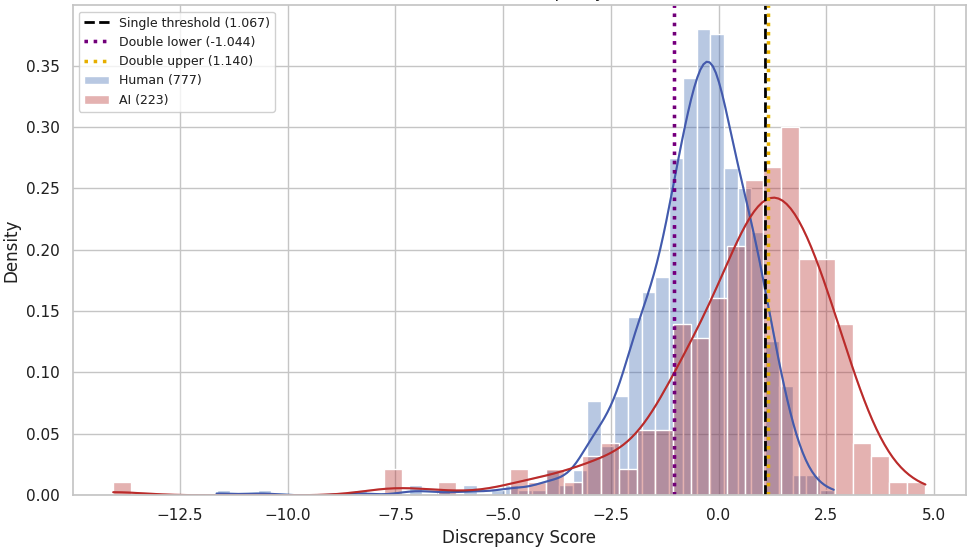
\includegraphics[width=\columnwidth]{assets/task_a_test.png}
  \caption{Single-threshold decision strategy on the official generic code test set using Stable-Code-3B.}
  \label{fig:threshold-test}
\end{figure}

This comparison highlights that the double-threshold rule is effective when the score distributions preserve a clear separation between the central human region and both machine-code tails. However, under domain shift, the lower tail becomes less discriminative because human-written code also appears in extreme negative-score regions. For this reason, the single-threshold strategy is more robust in the official test setting: it ignores the unstable lower tail and relies only on the upper discrepancy region, leading to the best overall Macro F1-score.


\subsection{Subtask B}

Table \ref{tab:overall_tB} reports the overall performance of our approach on Subtask B. The proposed UniXCoder-based achieves a Macro F1-score of 0.372, which is the official evaluation metric of the shared task, together with an overall accuracy of 67.7\%.
\begin{table}[h]
  \centering
  \small
  \caption{Performance on Subtask B.}
  \label{tab:overall_tB}
  \begin{tabular}{lc}
    \toprule
    \textbf{Metric} & \textbf{Score} \\
    \midrule
    Accuracy & 0.6770 \\
    Macro Precision & 0.3702 \\
    Macro Recall & 0.4012 \\
    Macro F1 & 0.3718 \\
    Weighted F1 & 0.6980 \\
    \bottomrule
  \end{tabular}
\end{table}

The results for individual classes are reported in Table \ref{tab:class_results}. The model performs particularly well on the \textit{human} and \textit{openai} classes, achieving F1-scores of 0.949 and 0.760, respectively. Among the remaining LLM families, \textit{gemma} and \textit{01-ai} obtain the strongest results, with F1-scores of 0.481 and 0.423. In contrast, performance on minority classes such as \textit{deepseek}, \textit{mistral}, and \textit{ibm-granite} remains considerably lower, highlighting the difficulty of distinguishing between less represented generator families.
\begin{table}[h]
  \centering
  \small
  \setlength{\tabcolsep}{4pt}
  \caption{Per-class performance on the Task B test set.}
  \label{tab:class_results}
  \begin{tabular}{lcccc}
    \toprule
    \textbf{Class} & \textbf{Precision} & \textbf{Recall} & \textbf{Macro F1} & \textbf{Support} \\
    \midrule
    Human & 0.9734 & 0.9262 & 0.9492 & 474 \\
    DeepSeek & 0.0545 & 0.1429 & 0.0789 & 21 \\
    Qwen & 0.2644 & 0.3151 & 0.2875 & 73 \\
    01-ai & 0.3548 & 0.5238 & 0.4231 & 21 \\
    BigCode & 0.2308 & 0.3000 & 0.2609 & 10 \\
    Gemma & 0.4419 & 0.5278 & 0.4810 & 36 \\
    Phi & 0.3056 & 0.2037 & 0.2444 & 54 \\
    Meta-LLaMA & 0.3143 & 0.1803 & 0.2292 & 61 \\
    IBM-Granite & 0.1522 & 0.3889 & 0.2188 & 18 \\
    Mistral & 0.1212 & 0.2222 & 0.1569 & 18 \\
    OpenAI & 0.8588 & 0.6822 & 0.7604 & 214 \\
    \midrule
    Macro Avg & 0.3702 & 0.4012 & 0.3718 & 1000 \\
    Weighted Avg & 0.7319 & 0.6770 & 0.6980 & 1000 \\
    \bottomrule
  \end{tabular}
\end{table}

Figure \ref{fig:norm_conf_matrix_tB} shows the normalized confusion matrix. While human-written code is correctly recognized in most cases, substantial confusion is observed among several LLM families. In particular, Qwen samples are frequently misclassified as Phi and OpenAI, whereas Meta-LLaMA exhibits notable overlap with Qwen, IBM-Granite, and Mistral. Similar confusion patterns can also be observed between IBM-Granite and Mistral. These results suggest that different LLM families often generate code with highly similar stylistic and structural characteristics, making fine-grained authorship attribution significantly more challenging than distinguishing between human-written and machine-generated code.
% \begin{figure}[h]
%   \centering
%   \includegraphics[width=0.45\textwidth]{assets/Confusion_Matrix_task_B.jpeg}
%   \caption{Confusion matrix obtained on the Subtask B test set.}
%   \label{fig:conf_matrix_tB}
% \end{figure}

\begin{figure}[h]
  \centering
  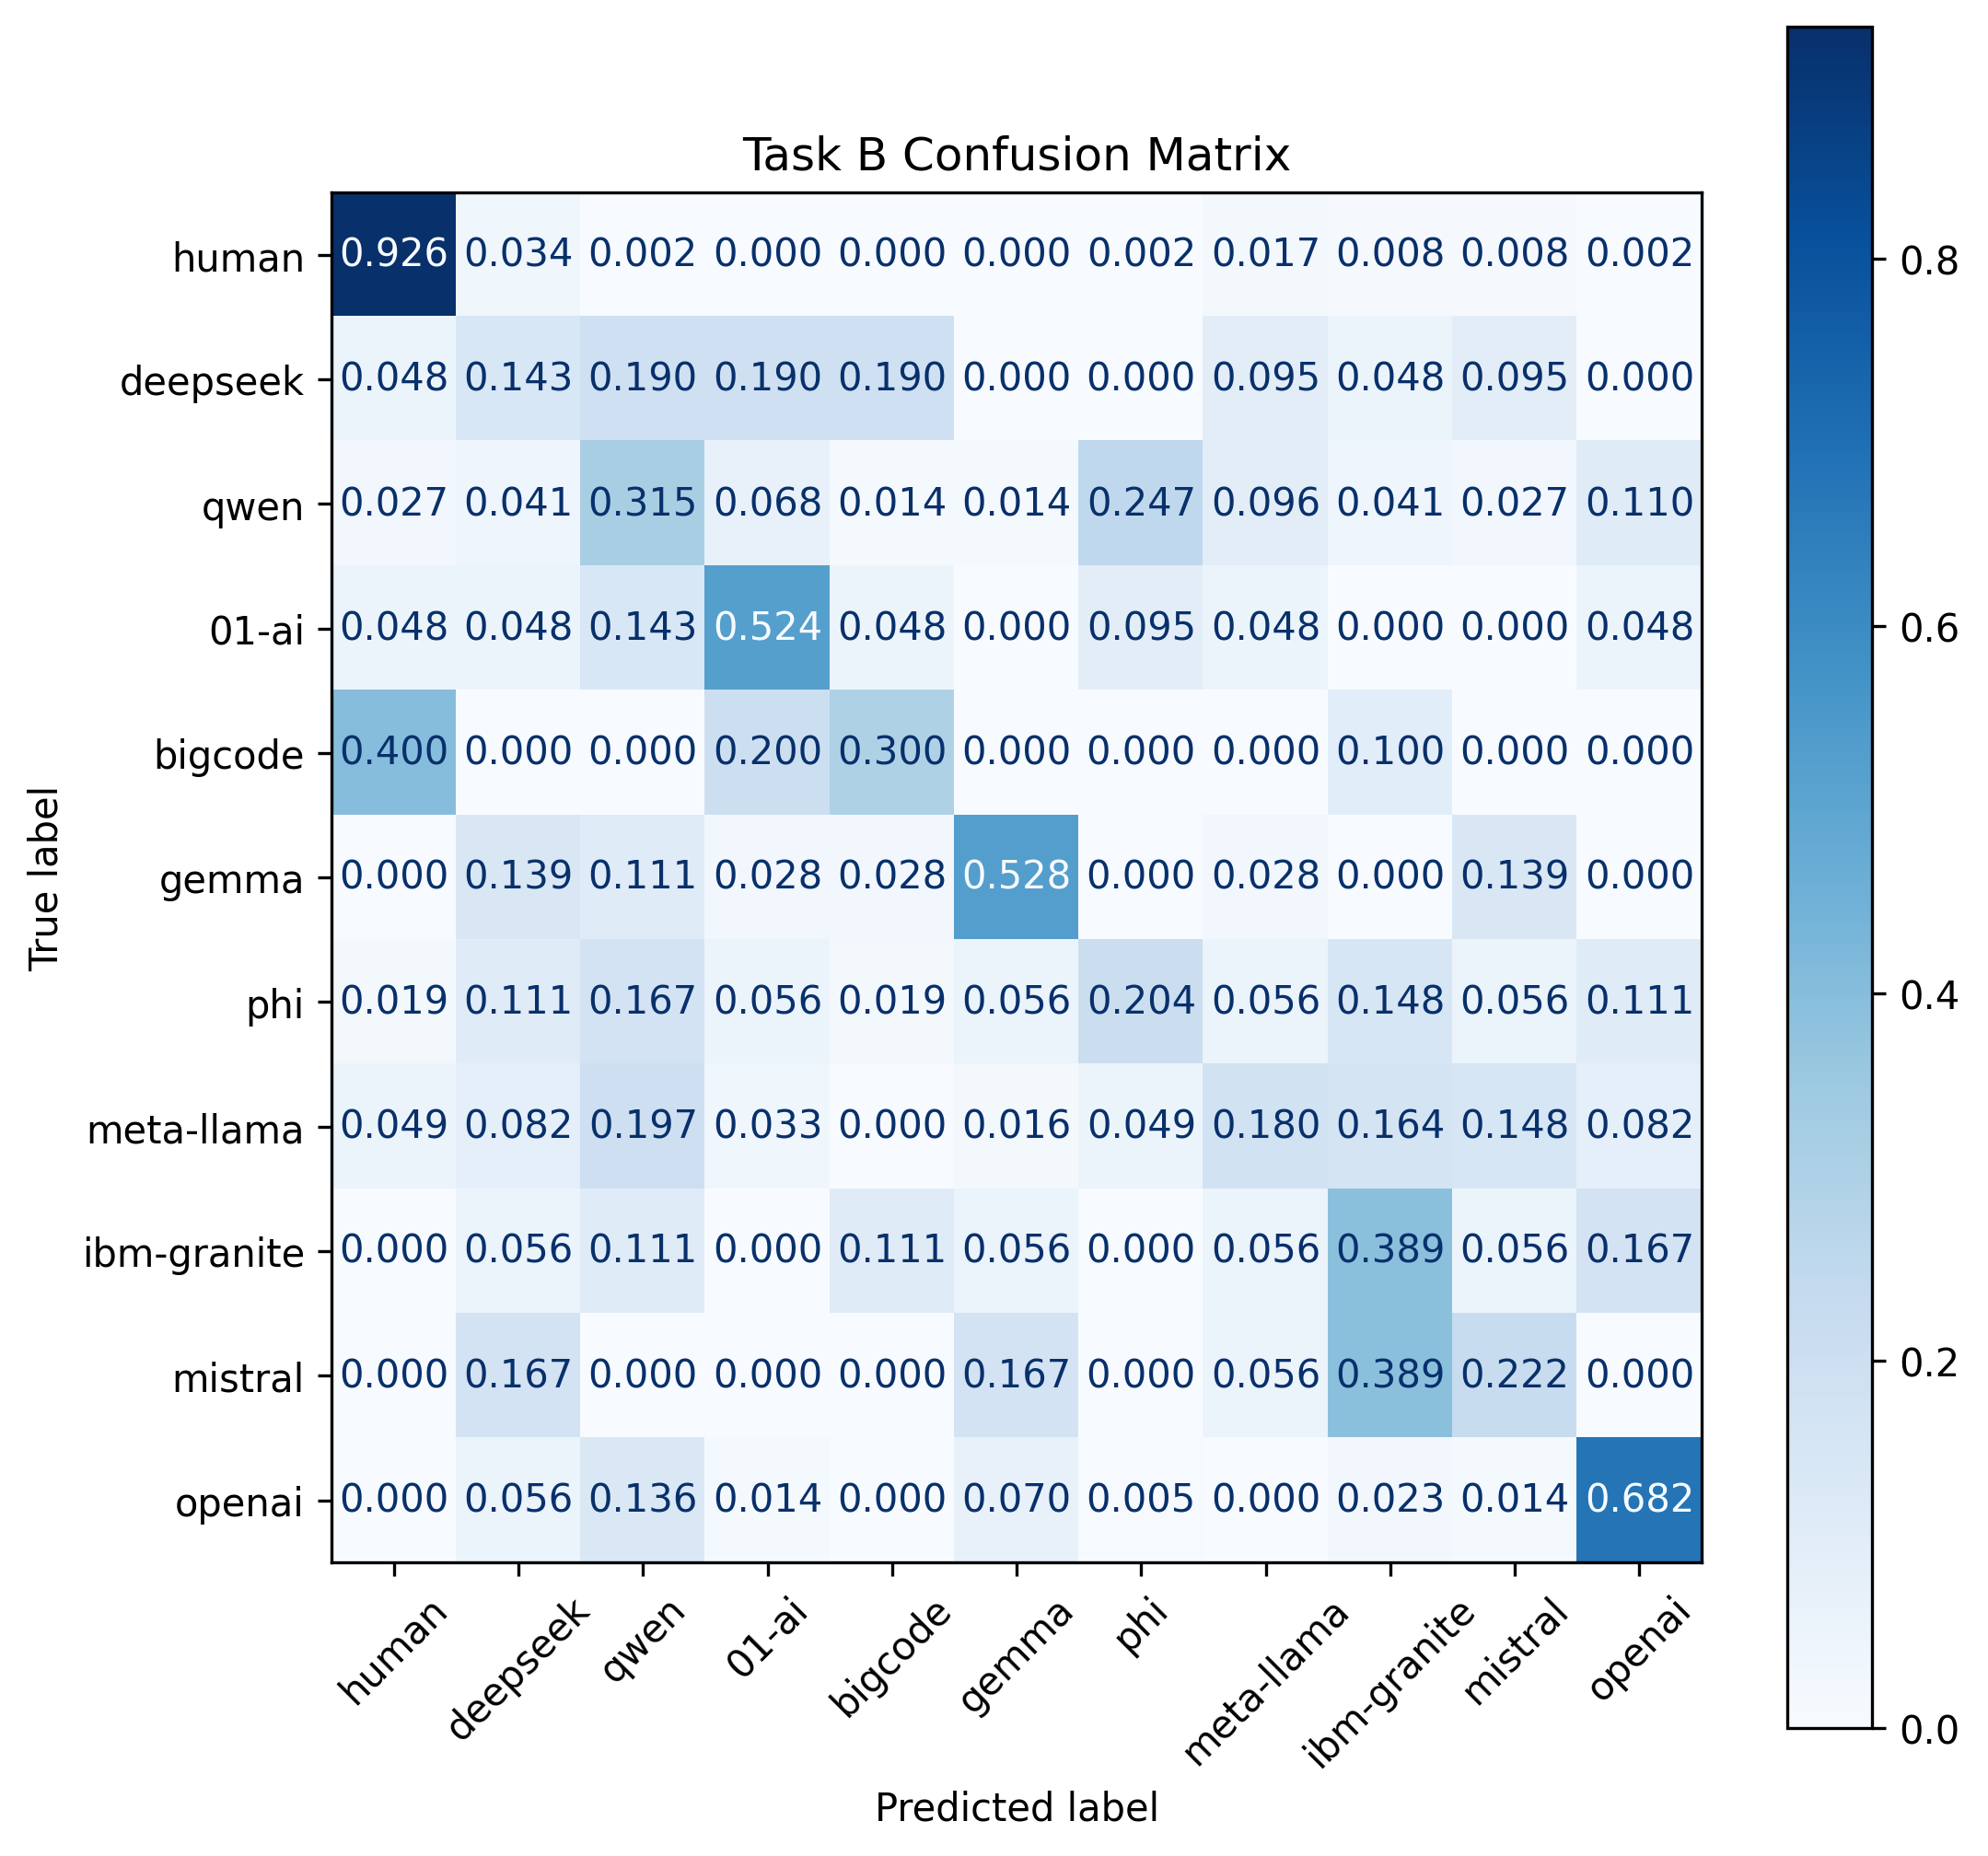
\includegraphics[width=0.45\textwidth]{assets/task_b_confusion_matrix_norm.png}
  \caption{Confusion matrix obtained on the Subtask B test set.}
  \label{fig:norm_conf_matrix_tB}
\end{figure}

Overall, the results indicate that the proposed approach effectively separates human and machine-generated code, but struggles to reliably discriminate among closely related LLM families, especially in the presence of severe class imbalance.

\subsection{Subtask C}

Table \ref{tab:class_results_tC} reports the overall and per-class performance of our fine-tuned UniXcoder model on the Subtask C test set. The proposed system achieved a strong overall Macro F1-score of 0.84 and a Accuracy of 88.70\%, demonstrating robust capability to identify complex generation artifacts even in the presence of code modifications.

% \begin{table}[h]
%   \centering
%   \caption{Overall and per-class performance on the Subtask C test set.}
%   \label{tab:class_results_tC}
%   \resizebox{\columnwidth}{!}{
%     \begin{tabular}{lcccc}
%       \hline
%       Class & Precision & Recall & F1-score & Support \\
%       \hline
%       Human & 0.9865 & 0.9224 & 0.9534 & 554 \\
%       Machine & 0.8810 & 0.8114 & 0.8447 & 228 \\
%       Hybrid & 0.7115 & 0.8810 & 0.7872 & 84 \\
%       Adversarial & 0.6964 & 0.8731 & 0.7748 & 134 \\
%       \hline
%       Macro Avg & 0.8189 & 0.8720 & 0.8400 & 1000 \\
%       Weighted Avg & 0.9005 & 0.8870 & 0.8907 & 1000 \\
%       \hline
%   \end{tabular}}
% \end{table}

\begin{table}[htbp]
  \centering
  \small
  \setlength{\tabcolsep}{4pt}
  \caption{Overall and per-class performance on the Subtask C test set.}
  \label{tab:class_results_tC}
  \begin{tabular}{lcccc}
    \toprule
    \textbf{Class} & \textbf{Precision} & \textbf{Recall} & \textbf{Macro F1} & \textbf{Support} \\
    \midrule
    Human & 0.9865 & 0.9224 & 0.9534 & 554 \\
    Machine & 0.8810 & 0.8114 & 0.8447 & 228 \\
    Hybrid & 0.7115 & 0.8810 & 0.7872 & 84 \\
    Adversarial & 0.6964 & 0.8731 & 0.7748 & 134 \\
    \midrule
    Accuracy & & & 0.8870 & 1000 \\
    Macro Avg & 0.8189 & 0.8720 & 0.8400 & 1000 \\
    Weighted Avg & 0.9005 & 0.8870 & 0.8907 & 1000 \\
    \bottomrule
  \end{tabular}
\end{table}

Performance was highest on the \textit{human} class (0.953 F1-score), followed by fully \textit{machine-generated} code (0.845 F1-score). Despite the inherent complexity of detecting partial alterations, the model reliably identified both \textit{hybrid} and \textit{adversarial} samples, achieving F1-scores of 0.787 and 0.775, respectively. Notably, the high recall for both hybrid (0.881) and adversarial (0.873) categories indicates that the class-weighted Focal Loss successfully prevented the network from ignoring these underrepresented, complex categories.

% \begin{figure}[h]
%   \centering
%   \includegraphics[width=0.45\textwidth]{assets/Confusion_Matrix_task_C.jpeg}
%   \caption{Normalized confusion matrix obtained on the Subtask C test set.}
%   \label{fig:conf_matrix_tC}
% \end{figure}

\begin{figure}[h]
  \centering
  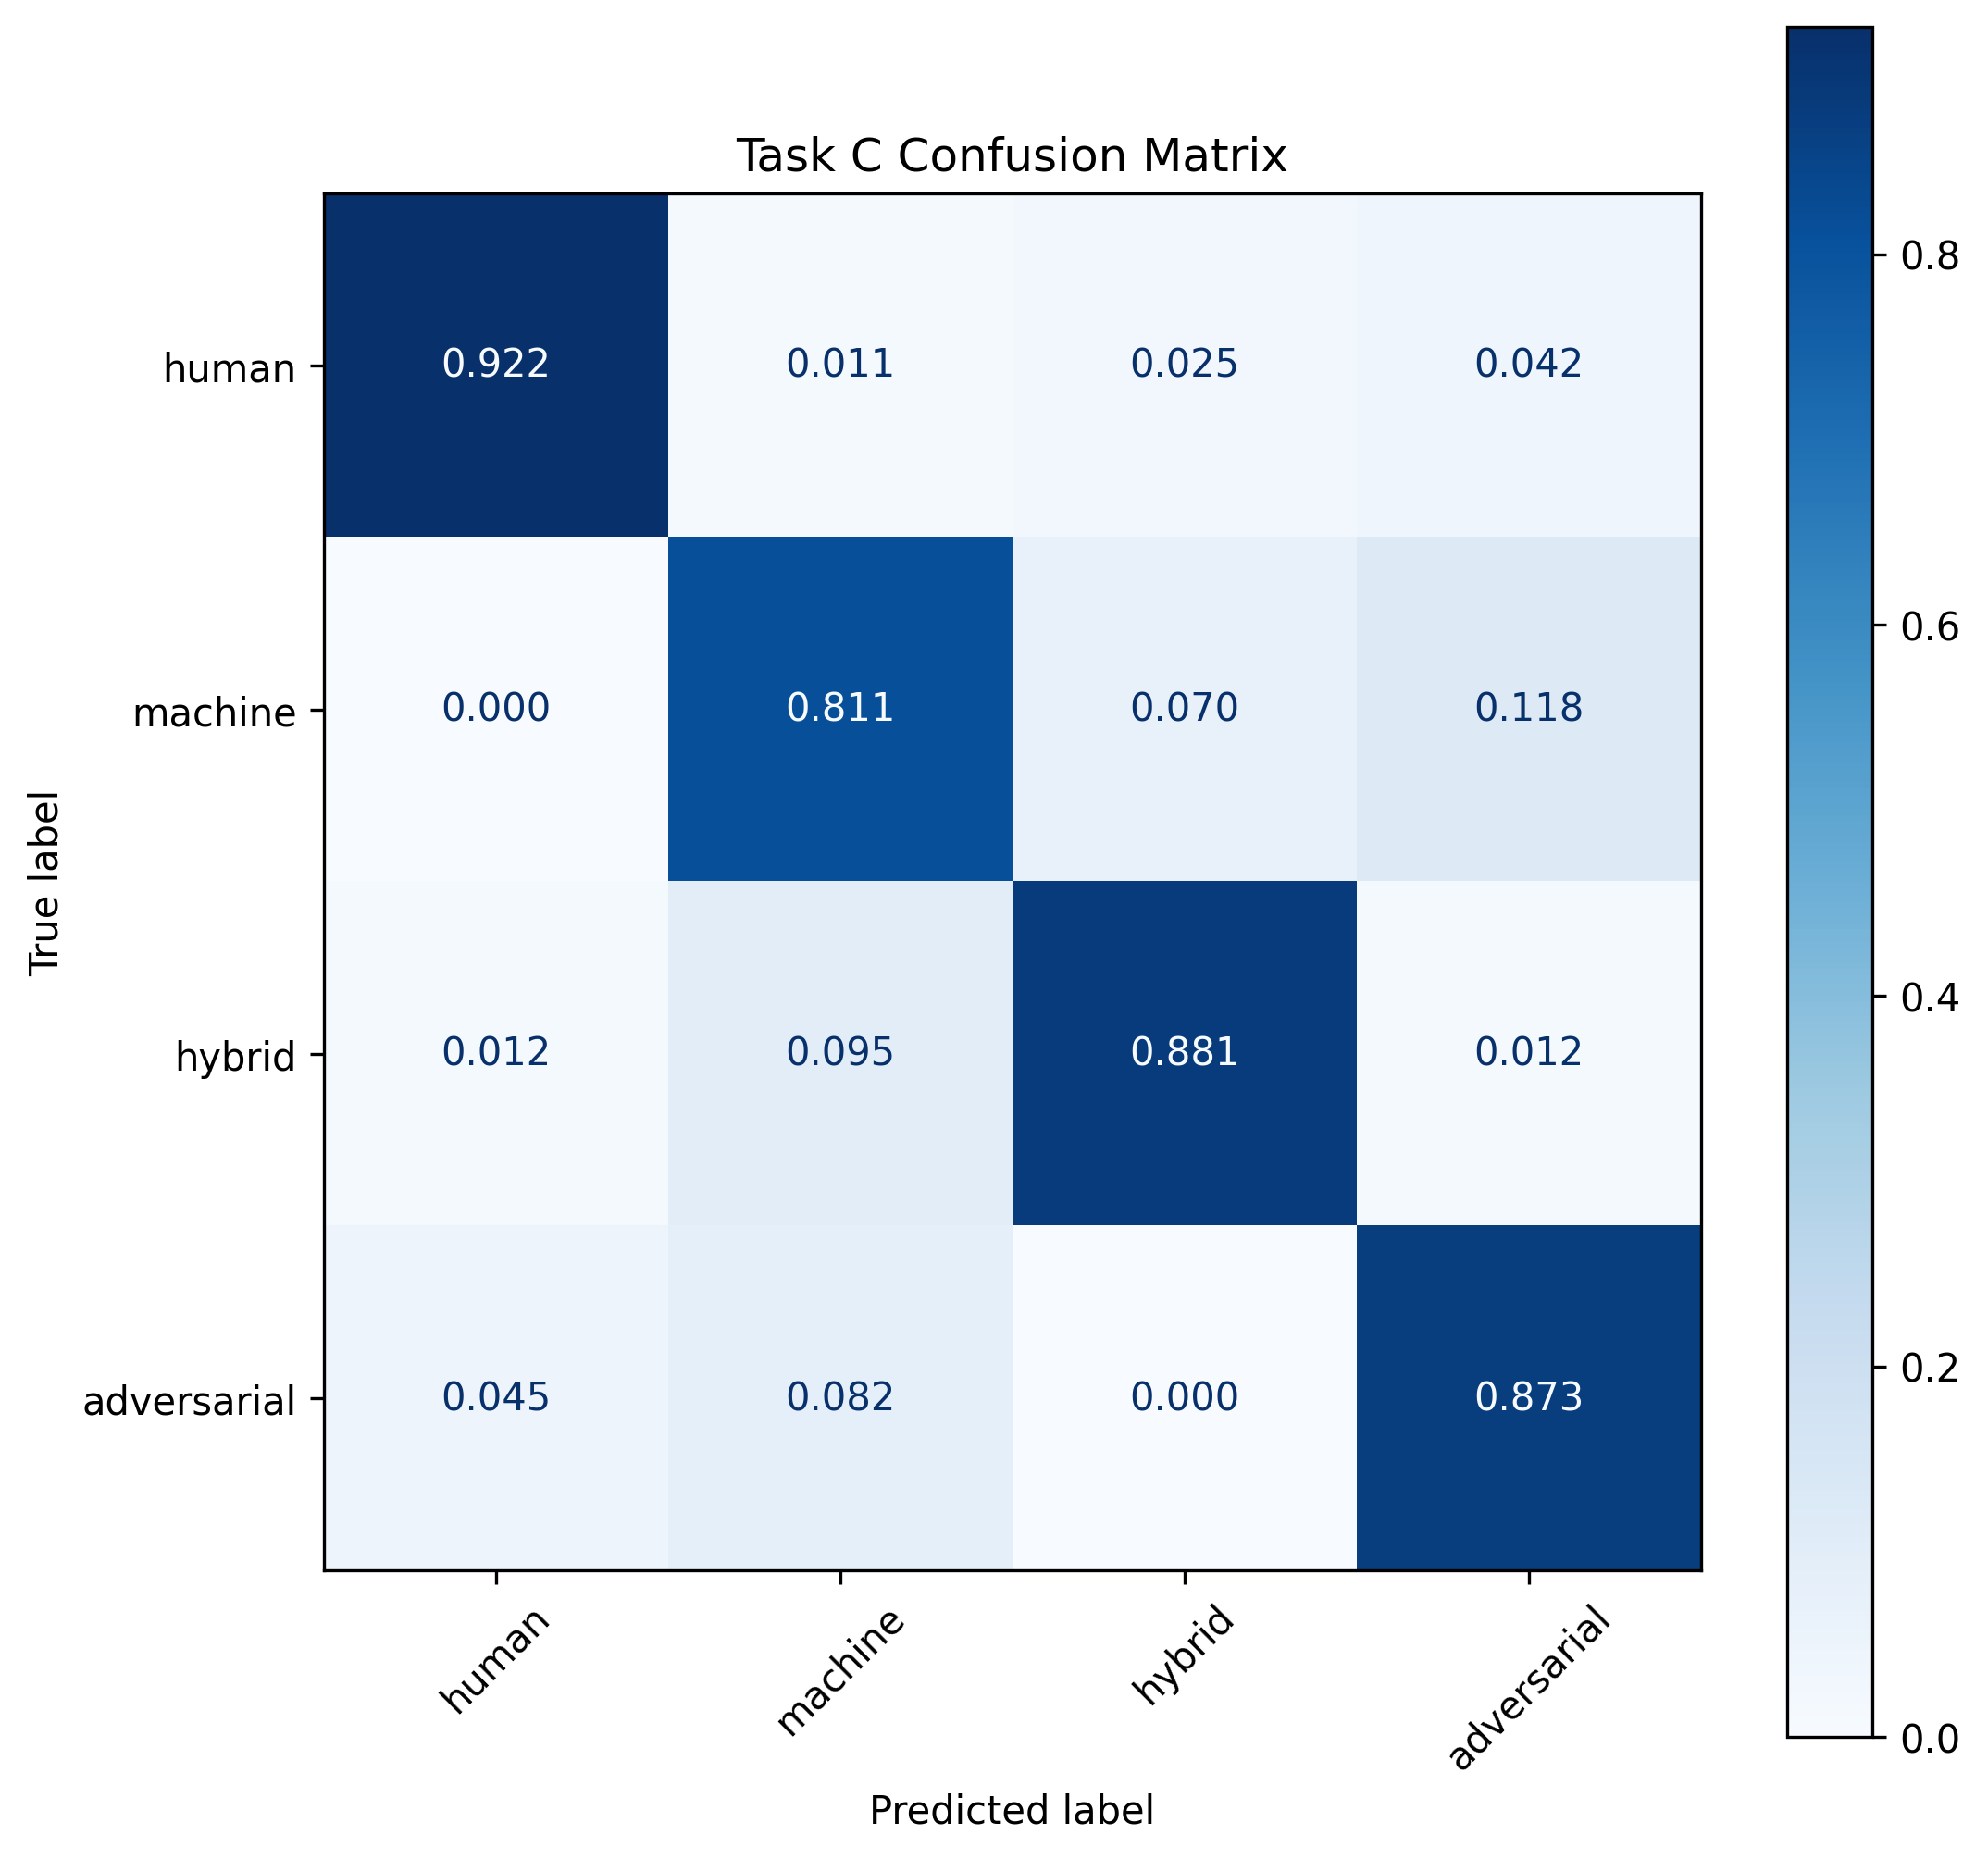
\includegraphics[width=0.35\textwidth]{assets/task_c_confusion_matrix_norm.png}
  \caption{Normalized confusion matrix obtained on the Subtask C test set.}
  \label{fig:norm_conf_matrix_tC}
\end{figure}

As illustrated in the normalized confusion matrix (Figure \ref{fig:norm_conf_matrix_tC}), human-written code is correctly identified in 92.2\% of cases. However, the matrix reveals logical overlap among the synthetic categories. Fully machine-generated code is occasionally misclassified as adversarial (11.8\%) or hybrid (7.0\%). Conversely, hybrid samples show a 9.5\% confusion rate with machine-generated code, and adversarial samples are sometimes mistaken for machine code (8.2\%) or human code (4.5\%). These patterns align with the intrinsic nature of the data, as adversarial and hybrid examples are intentionally engineered to mimic human stylometrics or blur attribution boundaries.

Overall, the results confirm that leveraging a deep semantic encoder like UniXcoder, paired with an class-weighted Focal Loss, provides a highly effective mechanism for isolating fine-grained generation and adversarial artifacts in source code.

\section{Conclusion}

This work presented complementary approaches for machine-generated code detection and authorship attribution across the SemEval-2026 Task 13 subtasks. For Subtask A, we adapted Fast-DetectGPT to source code and analyzed how different thresholding strategies behave across code domains. Our main finding is that threshold selection strongly depends on the target distribution. In the algorithmic LeetCode-style domain, the double-threshold strategy introduced in our work is preferable, since machine-generated code exhibits discriminative mass in both the upper and lower tails of the discrepancy-score distribution. In contrast, when moving to more generic code from production or research-oriented domains, the lower tail becomes less reliable and overlaps more with human-written samples. In this setting, the original single-threshold strategy provides a more robust decision boundary and achieves more consistent performance.

For Subtasks B and C, we relied on transformer-based classification models. By fine-tuning UniXCoder and incorporating class-weighted Focal Loss, our systems were able to learn discriminative representations of source code while partially mitigating the impact of class imbalance.

The experimental results highlight a clear difference in task difficulty. Subtask C demonstrates that transformer-based code representations are highly effective for distinguishing broad categories of code provenance, including human-written, machine-generated, hybrid, and adversarial samples. The confusion matrix shows a strong separation among the four classes, indicating that UniXCoder captures high-level authorship and generation characteristics even in the presence of adversarial modifications.

In contrast, Subtask B proved substantially more challenging. While the model successfully identified human-written code and some generator families, performance decreased when distinguishing among individual LLM families. The confusion matrix revealed significant overlap between several generators, suggesting that different LLMs often produce code with highly similar stylistic and structural patterns. This observation highlights the increased complexity of fine-grained authorship attribution compared to broader source classification, suggesting a substantial stylistic overlap among modern LLM families.

Overall, our findings indicate that transformer-based code representations are effective for general code provenance analysis, whereas attribution to specific model families remains an open challenge. A major limitation of our approach is the severe class imbalance present in the training data, which negatively affects minority classes despite the use of class-weighted Focal Loss. Future work could explore data augmentation, contrastive learning, ensemble methods, or larger code-oriented language models to improve robustness and  increase the separation between closely related LLM families.

\newpage
\bibliography{custom}

\end{document}

----
